% !TeX program = lualatex
% ================================================================
% Polish Parallel Text Version of TimesTablesToNthTerms
%
% Generated by the server using the following settings:
%
%   language            Polish (pol)
%   text direction      left to right
%   font                Noto Serif
%   fallback font       Noto Serif
%   built from          latex/worksheets/sequences/timesTablesToNthTerms.tex
%   vocabulary key      latex/worksheets/sequences/timesTablesToNthTerms/L2/pol/timesTablesToNthTerms_polishKey.tex
%   tier 3 vocabulary   green   RGB 0 128 0
%   English text        black   RGB 0 0 0
%   Polish text         purple  RGB 112 48 160
%   layout macros       version 3
%
% Please don't edit any information in this comment block - the server
% compares it against the current settings and rebuilds this file when
% they differ, so changes here would be overwritten. However, feel free
% to make updates to the LaTeX below if you want to edit it.
% ================================================================

\documentclass[11pt,a4paper]{article}
% ================================================================
% Copied from the English sheet this was translated from, so that
% anything it sets up for itself still works here
% ================================================================
\usepackage[a4paper,top=10mm,bottom=10mm,left=14mm,right=14mm]{geometry}
\usepackage[T1]{fontenc}
\usepackage{amsmath}
\usepackage{amssymb}
\usepackage{enumitem}
\usepackage{multicol}
\usepackage{array}
\usepackage{tikz}
\usepackage[most]{tcolorbox}
\usetikzlibrary{arrows.meta}

% ================================================================
% From times tables to the nth term.
%
% A first sheet on the nth term, built on what pupils already know
% about times tables. Part 1 lists times tables, moving from whole
% numbers on to decimals, fractions, percentages and negatives.
% Part 2 substitutes into expressions such as 3n, which are the same
% times tables written in algebra, and Part 3 matches sequences to
% their nth terms.
%
% Part 4 counts the objects in picture sequences and tabulates them.
% Part 5 matches picture sequences to their nth terms and ends with
% pupils drawing their own picture sequences.
%
% The sheet comes before the nth term is formally taught, so every
% picture sequence is a times table. Expressions such as n+4 appear
% only as the unused answers in the matching questions.
%
% Every picture is drawn from n by the macros below, so that the
% number of objects in each pattern is the value of the nth term.
% Part 6 is an optional fourth side of always, sometimes or never
% statements, which can be left out by printing the first three sides.
% The sheet is written on, and the main sheet is exactly three sides
% of A4.
% ================================================================

\pagestyle{empty}
\setlength{\parindent}{0pt}
\setlength{\parskip}{3pt}
\setlength{\multicolsep}{3pt}
\setlength{\columnsep}{14pt}
\setlist[enumerate,1]{label=\textbf{Q\arabic*.}, leftmargin=*, itemsep=5pt, topsep=3pt, parsep=2pt}
\setlist[enumerate,2]{label=(\alph*), leftmargin=*, itemsep=5pt, topsep=3pt, parsep=1pt}
\newcolumntype{C}[1]{>{\centering\arraybackslash}m{#1}}

% A gap for one term of a sequence.
\newcommand{\gap}{\underline{\hspace{0.95cm}}}
\newcommand{\ansline}[1][2.2cm]{\underline{\hspace{#1}}}
% The strut that sets the height of a table row to be written in.
\newcommand{\rowstrut}{\rule[-2mm]{0pt}{6.2mm}}

% The idea the sheet is built on, stated once and boxed. The box is
% tinted only faintly so that the sheet is cheap to print.
\newtcolorbox{keyidea}{colback=orange!2,colframe=orange!60!black,boxrule=0.6pt,
  left=6pt,right=6pt,top=2pt,bottom=2pt}

% The section headings, kept tight so the parts do not eat the page.
\newcommand{\parttitle}[2]{%
  \vspace{1pt}
  {\color{blue!45!black}\rule{\linewidth}{1pt}}\\[1pt]
  {\large\bfseries Part #1: #2}\\[-6pt]
  {\color{blue!45!black}\rule{\linewidth}{0.4pt}}
  \par\vspace{-5pt}}

% ----------------------------------------------------------------
% A grid for listing times tables, with one \ttrow for each times
% table: \ttrow{<times table>}{<six terms>}
\newenvironment{tablegrid}{%
  \setlength{\tabcolsep}{2pt}%
  \begin{tabular}{|C{1.05cm}|*{6}{C{1.05cm}|}}\hline
  {\small Table} & $\times1$ & $\times2$ & $\times3$ & $\times4$ & $\times5$ & $\times6$\\\hline}
  {\end{tabular}}
\newcommand{\ttrow}[7]{\textbf{#1} & #2 & #3 & #4 & #5 & #6 & #7\rowstrut\\\hline}

% A table for substituting into expressions, with one \subrow for each
% expression: \subrow{<expression>}{<six values>}{<times table>}
\newenvironment{subtable}{%
  \setlength{\tabcolsep}{3pt}%
  \begin{tabular}{|C{1.5cm}|*{6}{C{1.5cm}|}C{1.7cm}|}\hline
  $n$ & 1 & 2 & 3 & 4 & 5 & 10 & {\scriptsize Times table}\\\hline}
  {\end{tabular}}
\newcommand{\subrow}[8]{$#1$ & #2 & #3 & #4 & #5 & #6 & #7 & #8\rowstrut\\\hline}

% The table for a picture sequence, with one \picrow for each row.
% The last column holds the nth term.
\newenvironment{pictable}{%
  \setlength{\tabcolsep}{2pt}%
  \begin{tabular}{|C{1.85cm}|*{6}{C{0.74cm}|}C{1.75cm}|}\hline
  {\small Pattern $n$} & 1 & 2 & 3 & 4 & 5 & 10 & {\small $n$th term}\\\hline}
  {\end{tabular}}
\newcommand{\picrow}[1]{{\small #1} & & & & & & & \rowstrut\\\hline}

% A picture sequence on the left and its table on the right.
\newcommand{\pictureandtable}[2]{%
  \begin{minipage}[c]{0.42\linewidth}#1\end{minipage}\hfill
  \begin{minipage}[c]{0.57\linewidth}\raggedleft #2\end{minipage}}

% ----------------------------------------------------------------
% Picture sequences. In each of these the argument is the pattern
% number n.
\tikzset{
  stick/.style={line width=1.1pt,cap=round,shorten >=1.3pt,shorten <=1.3pt,
    -{Circle[length=3.2pt,width=3.2pt]}}}
\newcommand{\pic}[1]{\begin{tikzpicture}[baseline=(current bounding box.south)]#1\end{tikzpicture}}
% One matchstick from one point to another.
\newcommand{\stick}[2]{\draw[stick] (#1) -- (#2);}

% n rows of #2 dots.
\newcommand{\dotrows}[2]{\pic{%
  \foreach \i in {1,...,#2} \foreach \j in {1,...,#1}
    \fill (0.3*\i,0.3*\j) circle (0.075);}}

% n separate squares of matchsticks.
\newcommand{\sepsquares}[1]{\pic{%
  \foreach \k in {1,...,#1} {
    \begin{scope}[shift={(0.8*\k,0)}]
      \stick{0,0}{0.6,0}\stick{0.6,0}{0.6,0.6}\stick{0.6,0.6}{0,0.6}\stick{0,0.6}{0,0}
    \end{scope}}}}

% n separate hexagons of matchsticks.
\newcommand{\sephexagons}[1]{\pic{%
  \foreach \k in {1,...,#1} {
    \begin{scope}[shift={(0.92*\k,0)}]
      \foreach \a in {0,60,...,300} {\stick{\a:0.4}{\a+60:0.4}}
    \end{scope}}}}

% n separate houses of matchsticks.
\newcommand{\sephouses}[1]{\pic{%
  \foreach \k in {1,...,#1} {
    \begin{scope}[shift={(0.8*\k,0)}]
      \stick{0,0}{0.55,0}\stick{0.55,0}{0.55,0.55}\stick{0,0.55}{0,0}\stick{0,0.55}{0.55,0.55}
      \stick{0,0.55}{0.275,0.87}\stick{0.275,0.87}{0.55,0.55}
    \end{scope}}}}

% A zigzag of 2n matchsticks.
\newcommand{\zigzag}[1]{\pic{%
  \pgfmathtruncatemacro{\last}{2*#1-1}
  \foreach \j in {0,...,\last} {
    \pgfmathsetmacro{\ya}{0.6*mod(\j,2)}\pgfmathsetmacro{\yb}{0.6*mod(\j+1,2)}
    \stick{0.35*\j,\ya}{0.35*\j+0.35,\yb}}}}

% A row of n triangles of matchsticks that touch at their corners.
\newcommand{\toothtriangles}[1]{\pic{%
  \foreach \k in {1,...,#1} {
    \begin{scope}[shift={(0.7*\k,0)}]
      \stick{0,0}{0.7,0}\stick{0,0}{0.35,0.6}\stick{0.35,0.6}{0.7,0}
    \end{scope}}}}

% n dice, each showing a five.
\newcommand{\dicefives}[1]{\pic{%
  \foreach \k in {1,...,#1} {
    \begin{scope}[shift={(0.68*\k,0)}]
      \draw[thick,rounded corners=2pt] (0,0) rectangle (0.58,0.58);
      \foreach \x/\y in {0.14/0.14,0.44/0.14,0.29/0.29,0.14/0.44,0.44/0.44}
        \fill (\x,\y) circle (0.055);
    \end{scope}}}}

% n flowers of dots, each with a centre dot and six around it.
\newcommand{\dotflowers}[1]{\pic{%
  \foreach \k in {1,...,#1} {
    \begin{scope}[shift={(0.8*\k,0)}]
      \fill (0,0) circle (0.055);
      \foreach \a in {0,60,...,300} \fill (\a:0.22) circle (0.055);
    \end{scope}}}}

% A cross of dots with four arms of n dots.
\newcommand{\dotcross}[1]{\pic{%
  \foreach \i in {1,...,#1} \foreach \a in {0,90,180,270}
    \fill (\a:0.2*\i) circle (0.065);}}

% A star of dots with three arms of n dots.
\newcommand{\dotstar}[1]{\pic{%
  \foreach \i in {1,...,#1} \foreach \a in {90,210,330}
    \fill (\a:0.2*\i) circle (0.065);}}

% n separate square tables, each with four chairs. Each dot is a chair.
\newcommand{\septables}[1]{\pic{%
  \foreach \k in {1,...,#1} {
    \begin{scope}[shift={(0.86*\k,0)}]
      \draw[thick,sharp corners] (0,0) rectangle (0.4,0.4);
      \fill (0.2,-0.13) circle (0.07);
      \fill (0.2,0.53) circle (0.07);
      \fill (-0.13,0.2) circle (0.07);
      \fill (0.53,0.2) circle (0.07);
    \end{scope}}}}

% Patterns 1, 2 and 3 of a picture sequence, labelled underneath.
\newcommand{\threepatterns}[3]{%
  \begin{tabular}{@{}c@{\hspace{11pt}}c@{\hspace{11pt}}c@{}}
    #1 & #2 & #3\\[-1pt]
    {\scriptsize Pattern 1} & {\scriptsize Pattern 2} & {\scriptsize Pattern 3}
  \end{tabular}}

% ----------------------------------------------------------------
% A table of always, sometimes or never statements, carrying on the
% question numbers. \asnrow[<picture>]{<statement>}
\newcounter{asn}
\newcommand{\pill}[1]{\tikz[baseline=(x.base)]\node[draw=gray!70,rounded corners=6pt,
  inner sep=2.5pt,font=\small] (x) {#1};}
\newcommand{\pills}{\pill{Always}\ \pill{Sometimes}\ \pill{Never}}
\newenvironment{asntable}{%
  \setlength{\tabcolsep}{4pt}%
  \begin{tabular}{|>{\raggedright\arraybackslash}m{8.6cm}|m{8.9cm}|}\hline
  \textbf{Statement} & \textbf{Reason}\\\hline}
  {\end{tabular}}
\newcommand{\asnrow}[2][]{\stepcounter{asn}%
  \rule{0pt}{4mm}\textbf{Q\theasn.} #2\par\vspace{3pt}\pills\hfill #1
  & \rule{0pt}{1.5cm}\\\hline}

% Dotted paper to draw a picture sequence on, with a box around it.
\newcommand{\dotpaper}[2]{%
  \begin{tikzpicture}[baseline=(current bounding box.north)]
    \foreach \x in {0.25,0.75,...,#1} \foreach \y in {0.25,0.75,...,#2}
      \fill[gray!60] (\x,\y) circle (0.024);
    \draw[gray!60] (0,0) rectangle (#1,#2);
  \end{tikzpicture}}

% Characters this language's font has not got are borrowed from another,
% rather than being silently dropped - see docs/translated-sheet-latex.md
\directlua{%
  if luaotfload and luaotfload.add_fallback then
    luaotfload.add_fallback("eallatinfallback",
      { "Noto Serif:mode=harf;" })
  else
    tex.error("this luaotfload is too old to register a fallback font")
  end
}
\usepackage[english]{babel}
\babelprovide[import]{polish}
\babelfont[polish]{rm}[Renderer=Harfbuzz, BoldFont={Noto Serif}, ItalicFont={Noto Serif}, BoldItalicFont={Noto Serif}, RawFeature={fallback=eallatinfallback}]{Noto Serif}
\babelfont[polish]{sf}[Renderer=Harfbuzz, BoldFont={Noto Serif}, ItalicFont={Noto Serif}, BoldItalicFont={Noto Serif}, RawFeature={fallback=eallatinfallback}]{Noto Serif}
\newcommand{\ealtext}[1]{\foreignlanguage{polish}{#1}}
\newcommand{\ealtextblock}[1]{{\raggedright\foreignlanguage{polish}{#1}\par}}
% ================================================================
% EAL layout helpers
% ================================================================
\usepackage{xcolor}

\definecolor{ealkeycolour}{RGB}{0,128,0}
\definecolor{ealenglish}{RGB}{0,0,0}
\definecolor{ealtwocolour}{RGB}{112,48,160}

\newsavebox{\ealboxen}
\newsavebox{\ealboxtr}
\newlength{\ealglosswd}
\newlength{\ealglossraise}
\setlength{\ealglossraise}{1.15em}

% a tier 3 word, in English and in translation alike
\newcommand{\ealkey}[1]{\textcolor{ealkeycolour}{#1}}
\newcommand{\ealkeytr}[1]{\textcolor{ealkeycolour}{\ealtext{#1}}}

% One translated word above one English word. Built from kernel
% primitives, never a tabular, which would break wherever the sheet
% loads array, booktabs or tabularx. The box is as wide as the wider of
% the two, so a long translation pushes its neighbours aside instead of
% overlapping them, and it claims its full height so a table row or a
% TikZ node makes room for it.
\newcommand{\ealgloss}[2]{%
  \sbox{\ealboxen}{\ealkey{#1}}%
  \sbox{\ealboxtr}{\small\textcolor{ealtwocolour}{\ealtext{#2}}}%
  \setlength{\ealglosswd}{\wd\ealboxen}%
  \ifdim\wd\ealboxtr>\ealglosswd\setlength{\ealglosswd}{\wd\ealboxtr}\fi
  \leavevmode
  \makebox[\ealglosswd][c]{%
    \makebox[0pt][c]{\usebox{\ealboxen}}%
    \makebox[0pt][c]{\raisebox{\ealglossraise}{\usebox{\ealboxtr}}}%
  }%
}

% opens up line spacing around a block of glosses, so the raised
% translations sit clear of the line above
\newenvironment{ealglossed}{\par\linespread{2.1}\selectfont\ignorespaces}{\par}

% a whole translated sentence above its English counterpart. block level,
% so it does not belong inside a tabular cell
\newcommand{\ealpara}[2]{%
  \par\addvspace{0.5\baselineskip}%
  {\color{ealtwocolour}\ealtextblock{#1}}%
  \penalty200
  {\color{ealenglish}#2\par}%
  \addvspace{0.5\baselineskip}%
}

\begin{document}

\begin{center}
  {\Large\bfseries \ealpara{Od \ealkeytr{tabliczek mnożenia} do \ealkeytr{wzoru na n-ty wyraz}}{From \ealkey{Times Tables} to the \ealkey{\boldmath$n$th Term}}}
\end{center}
\vspace{6pt}

\parttitle{1}{\ealkey{Times tables}}

\begin{enumerate}
\item \ealpara{Zapisz pierwsze sześć \ealkeytr{wyrazów} każdej \ealkeytr{tabliczki mnożenia}.}{Write the first six \ealkey{terms} of each \ealkey{times table}.}

\begin{tablegrid}
\ttrow{2}{2}{4}{}{}{}{}
\ttrow{5}{5}{10}{}{}{}{}
\ttrow{3}{3}{}{}{}{}{}
\end{tablegrid}\hfill
\begin{tablegrid}
\ttrow{7}{7}{}{}{}{}{}
\ttrow{12}{}{}{}{}{}{}
\ttrow{15}{}{}{}{}{}{}
\end{tablegrid}

\item \ealpara{Zapisz pierwsze sześć \ealkeytr{wyrazów} każdej \ealkeytr{tabliczki mnożenia} \ealkeytr{ułamków dziesiętnych}.}{Write the first six \ealkey{terms} of each \ealkey{decimal} \ealkey{times table}.}

\begin{tablegrid}
\ttrow{0.1}{0.1}{0.2}{}{}{}{}
\ttrow{0.5}{0.5}{1}{}{}{}{}
\end{tablegrid}\hfill
\begin{tablegrid}
\ttrow{1.5}{1.5}{}{}{}{}{}
\ttrow{0.25}{}{}{}{}{}{}
\end{tablegrid}

\item \ealpara{Zapisz pierwsze sześć \ealkeytr{wyrazów} każdej \ealkeytr{tabliczki mnożenia} \ealkeytr{ułamków}, w \ealkeytr{najprostszej postaci}.}{Write the first six \ealkey{terms} of each \ealkey{fraction} \ealkey{times table}, in their \ealkey{simplest form}.}

\begin{tablegrid}
\ttrow{$\tfrac12$}{$\tfrac12$}{1}{}{}{}{}
\ttrow{$\tfrac14$}{$\tfrac14$}{$\tfrac12$}{}{}{}{}
\end{tablegrid}\hfill
\begin{tablegrid}
\ttrow{$\tfrac13$}{$\tfrac13$}{}{}{}{}{}
\ttrow{$\tfrac34$}{}{}{}{}{}{}
\end{tablegrid}

\item \ealpara{Zapisz pierwsze sześć \ealkeytr{wyrazów} każdej \ealkeytr{tabliczki mnożenia} \ealkeytr{procentów}.}{Write the first six \ealkey{terms} of each \ealkey{percentage} \ealkey{times table}.}

\begin{tablegrid}
\ttrow{10\%}{10\%}{20\%}{}{}{}{}
\ttrow{25\%}{25\%}{}{}{}{}{}
\end{tablegrid}\hfill
\begin{tablegrid}
\ttrow{5\%}{}{}{}{}{}{}
\ttrow{\small 12.5\%}{}{}{}{}{}{}
\end{tablegrid}

\item \ealpara{Zapisz pierwsze sześć \ealkeytr{wyrazów} każdej \ealkeytr{tabliczki mnożenia} liczb \ealkeytr{ujemnych}.}{Write the first six \ealkey{terms} of each \ealkey{negative} \ealkey{times table}.}

\begin{tablegrid}
\ttrow{$-2$}{$-2$}{$-4$}{}{}{}{}
\ttrow{$-5$}{$-5$}{}{}{}{}{}
\end{tablegrid}\hfill
\begin{tablegrid}
\ttrow{$-0.5$}{}{}{}{}{}{}
\ttrow{$-\tfrac14$}{}{}{}{}{}{}
\end{tablegrid}

\item \ealpara{Każda lista jest częścią \ealkeytr{tabliczki mnożenia}. Uzupełnij luki i zapisz, która to \ealkeytr{tabliczka mnożenia}.}{Each list is part of a \ealkey{times table}. Fill in the gaps and write which \ealkey{times table} it is.}
\begin{multicols}{2}
\begin{enumerate}
\item \ealpara{9, 18, \gap, 36 \hfill \ealkeytr{Tabliczka mnożenia}:}{9, 18, \gap, 36 \hfill \ealkey{Times table}:}
\noindent\ansline[1.2cm]
\item \ealpara{0.7, \gap, 2.1, 2.8 \hfill \ealkeytr{Tabliczka mnożenia}:}{0.7, \gap, 2.1, 2.8 \hfill \ealkey{Times table}:}
\noindent\ansline[1.2cm]
\item \ealpara{$\tfrac15$, \gap, $\tfrac35$, \gap \hfill \ealkeytr{Tabliczka mnożenia}:}{$\tfrac15$, \gap, $\tfrac35$, \gap \hfill \ealkey{Times table}:}
\noindent\ansline[1.2cm]
\item \ealpara{\gap, $-12$, $-18$, \gap \hfill \ealkeytr{Tabliczka mnożenia}:}{\gap, $-12$, $-18$, \gap \hfill \ealkey{Times table}:}
\noindent\ansline[1.2cm]
\end{enumerate}
\end{multicols}

\item \ealpara{Uzupełnij tabelę. Następnie zapisz, jaką \ealkeytr{tabliczkę mnożenia} daje każda sytuacja.}{Complete the table. Then write which \ealkey{times table} each situation gives.}
\ealpara{Liczba biletów, minut lub godzin}{Number of tickets, minutes or hours}
\ealpara{Koszt biletów do kina po \pounds7.50 każdy}{Cost of cinema tickets at \pounds7.50 each}
\ealpara{Wysokość nad poziomem morza łodzi podwodnej opuszczającej się o 30\,m każdą minutę}{Height above sea level of a submarine going down 30\,m each minute}
\ealpara{Bateria zużywana przez telefon, który zużywa 15\% naładowania każdą godzinę}{Battery used by a phone that uses 15\% of its charge each hour}

\setlength{\tabcolsep}{3pt}
\begin{tabular}{|>{\raggedright\arraybackslash}m{7.4cm}|*{5}{C{1.3cm}|}C{1.2cm}|}\hline
\small Number of tickets, minutes or hours & 1 & 2 & 3 & 4 & 5 & {\small Table}\\\hline
\small Cost of cinema tickets at \pounds7.50 each\rowstrut & & & & & & \\\hline
\small Height above sea level of a submarine going down 30\,m each minute\rowstrut & & & & & & \\\hline
\small Battery used by a phone that uses 15\% of its charge each hour\rowstrut & & & & & & \\\hline
\end{tabular}
\end{enumerate}

\parttitle{2}{\ealkey{Substituting} into \ealkey{expressions}}

\begin{keyidea}
\ealpara{W \ealkeytr{algebrze} $3n$ oznacza $3\times n$. Gdy $n=4$, \ealkeytr{podstawiamy}, aby otrzymać $3n=3\times4=12$.}{In \ealkey{algebra} $3n$ means $3\times n$. When $n=4$ we \ealkey{substitute} to get $3n=3\times4=12$.}
\end{keyidea}

\begin{enumerate}[resume]
\item \ealpara{\ealkeytr{Podstaw} każdą wartość $n$, aby uzupełnić tabelę. Następnie zapisz, jaką \ealkeytr{tabliczkę mnożenia} daje każde \ealkeytr{wyrażenie}.}{\ealkey{Substitute} each value of $n$ to complete the table. Then write which \ealkey{times table} each \ealkey{expression} gives.}

\begin{subtable}
\subrow{2n}{2}{4}{}{}{}{}{2}
\subrow{3n}{3}{}{}{}{}{}{}
\subrow{7n}{}{}{}{}{}{}{}
\subrow{12n}{}{}{}{}{}{}{}
\end{subtable}

\newpage
\item \ealpara{Zrób to samo dla tych \ealkeytr{wyrażeń}. Tutaj $5n\%$ oznacza $(5\times n)\%$.}{Do the same for these \ealkey{expressions}. Here $5n\%$ means $(5\times n)\%$.}

\begin{subtable}
\subrow{0.1n}{0.1}{}{}{}{}{}{}
\subrow{0.5n}{}{}{}{}{}{}{}
\subrow{\tfrac14n}{}{}{}{}{}{}{}
\subrow{5n\%}{}{}{}{}{}{}{}
\subrow{-2n}{}{}{}{}{}{}{}
\subrow{-0.5n}{}{}{}{}{}{}{}
\end{subtable}

\item \ealpara{Znajdź każdy \ealkeytr{wyraz}, \ealkeytr{podstawiając}. Nie wypisuj \ealkeytr{wyrazów}.}{Find each \ealkey{term} by \ealkey{substituting}. Do not list the \ealkey{terms}.}
\begin{multicols}{2}
\begin{enumerate}
\item \ealpara{Setny \ealkeytr{wyraz} $7n$:}{The 100th \ealkey{term} of $7n$:}
\noindent\ansline
\item \ealpara{Setny \ealkeytr{wyraz} $0.5n$:}{The 100th \ealkey{term} of $0.5n$:}
\noindent\ansline
\item \ealpara{Dwudziesty \ealkeytr{wyraz} $-3n$:}{The 20th \ealkey{term} of $-3n$:}
\noindent\ansline
\item \ealpara{Czy 60 jest \ealkeytr{wyrazem} \ealkeytr{ciągu} $7n$? Wyjaśnij.}{Is 60 a \ealkey{term} of the \ealkey{sequence} $7n$? Explain.}
\noindent\ansline[7cm]
\end{enumerate}
\end{multicols}
\end{enumerate}

\parttitle{3}{Matching \ealkey{sequences} to their \ealkey{$n$th terms}}

\begin{keyidea}
\ealpara{Lista liczb, która podlega regule, to \ealkeytr{ciąg}. Każda liczba na liście to \ealkeytr{wyraz}, a $n$ to \ealkeytr{pozycja} tego \ealkeytr{wyrazu} na liście. \ealkeytr{Wyrażenie}, które daje \ealkeytr{wyraz} na \ealkeytr{pozycji} $n$, to \ealkeytr{wzór na n-ty wyraz}.}{A list of numbers that follows a rule is a \ealkey{\textbf{sequence}}. Each number in the list is a \ealkey{\textbf{term}}, and $n$ is the \ealkey{\textbf{position}} of the \ealkey{term} in the list. The \ealkey{expression} that gives the \ealkey{term} at \ealkey{position} $n$ is the \ealkey{\textbf{$n$th term}}.}
\end{keyidea}

\begin{enumerate}[resume]
\item
\begin{enumerate}
\item \ealpara{Narysuj linię od każdego \ealkeytr{ciągu} do jego \ealkeytr{wzoru na n-ty wyraz}. Dwa \ealkeytr{wzory na n-ty wyraz} pozostają.}{Draw a line from each \ealkey{sequence} to its \ealkey{$n$th term}. Two \ealkey{$n$th terms} are left over.}

\begin{center}
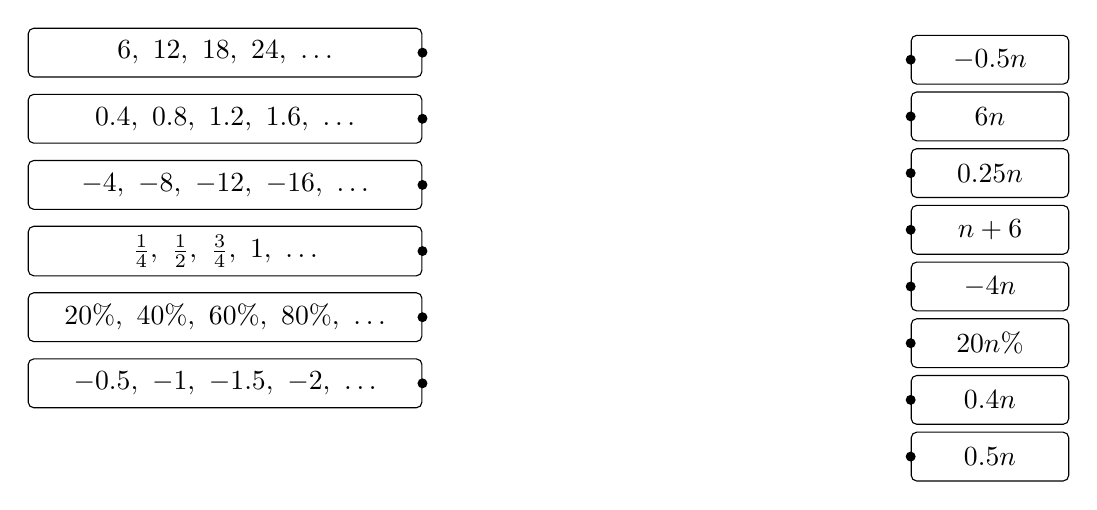
\begin{tikzpicture}[tile/.style={draw,rounded corners=2pt,minimum height=0.62cm,inner sep=3pt}]
  \foreach \y/\s in {
    1/{$6,\ 12,\ 18,\ 24,\ \ldots$},
    2/{$0.4,\ 0.8,\ 1.2,\ 1.6,\ \ldots$},
    3/{$-4,\ -8,\ -12,\ -16,\ \ldots$},
    4/{$\tfrac14,\ \tfrac12,\ \tfrac34,\ 1,\ \ldots$},
    5/{$20\%,\ 40\%,\ 60\%,\ 80\%,\ \ldots$},
    6/{$-0.5,\ -1,\ -1.5,\ -2,\ \ldots$}} {
    \node[tile,minimum width=5cm,anchor=east] (L\y) at (0,{-0.84*\y}) {\s};
    \fill (L\y.east) circle (1.8pt);}
  \foreach \y/\s in {
    1/{$-0.5n$}, 2/{$6n$}, 3/{$0.25n$}, 4/{$n+6$},
    5/{$-4n$}, 6/{$20n\%$}, 7/{$0.4n$}, 8/{$0.5n$}} {
    \node[tile,minimum width=2cm,anchor=west] (R\y) at (6.2,{-0.21-0.72*\y}) {\s};
    \fill (R\y.west) circle (1.8pt);}
\end{tikzpicture}
\end{center}

\item \ealpara{Zapisz pierwsze cztery \ealkeytr{wyrazy} każdego z dwóch \ealkeytr{wzorów na n-ty wyraz}, które pozostały.}{Write the first four \ealkey{terms} of each of the two \ealkey{$n$th terms} that are left over.}
\noindent\ansline[8cm]\hfill\ansline[8cm]
\end{enumerate}
\end{enumerate}

\parttitle{4}{Picture \ealkey{sequences}}

\begin{enumerate}[resume]
\item \ealpara{Policz obiekty w każdym wzorze i uzupełnij tabelę. Oblicz wzory 4, 5 i 10 bez rysowania ich. Następnie zapisz \ealkeytr{wzór na n-ty wyraz}.}{Count the objects in each pattern and complete the table. Work out patterns 4, 5 and 10 without drawing them. Then write the \ealkey{$n$th term}.}
\begin{enumerate}
\item \pictureandtable{\threepatterns{\dotrows{1}{3}}{\dotrows{2}{3}}{\dotrows{3}{3}}}%
  {\begin{pictable}\picrow{Dots}\end{pictable}}
\item \pictureandtable{\threepatterns{\sepsquares{1}}{\sepsquares{2}}{\sepsquares{3}}}%
  {\begin{pictable}\picrow{Matchsticks}\end{pictable}}
\item \pictureandtable{\threepatterns{\sephexagons{1}}{\sephexagons{2}}{\sephexagons{3}}}%
  {\begin{pictable}\picrow{Matchsticks}\end{pictable}}
\end{enumerate}

\newpage
\item \ealpara{Te wzory są ułożone inaczej, ale każdy z nich nadal jest \ealkeytr{tabliczką mnożenia}. Uzupełnij tabelę i zapisz \ealkeytr{wzór na n-ty wyraz}.}{These patterns are arranged differently, but each one is still a \ealkey{times table}. Complete the table and write the \ealkey{$n$th term}.}
\begin{enumerate}
\item \pictureandtable{\threepatterns{\zigzag{1}}{\zigzag{2}}{\zigzag{3}}}%
  {\begin{pictable}\picrow{Matchsticks}\end{pictable}}
\item \pictureandtable{\threepatterns{\toothtriangles{1}}{\toothtriangles{2}}{\toothtriangles{3}}}%
  {\begin{pictable}\picrow{Matchsticks}\end{pictable}}
\item \pictureandtable{\threepatterns{\dotcross{1}}{\dotcross{2}}{\dotcross{3}}}%
  {\begin{pictable}\picrow{Dots}\end{pictable}}
\end{enumerate}
\end{enumerate}

\parttitle{5}{Matching and drawing picture \ealkey{sequences}}

\begin{enumerate}[resume]
\item \ealpara{Narysuj linię od każdego \ealkeytr{ciągu} obrazkowego do jego \ealkeytr{wzoru na n-ty wyraz}. Trzy \ealkeytr{wzory na n-ty wyraz} pozostają.}{Draw a line from each picture \ealkey{sequence} to its \ealkey{$n$th term}. Three \ealkey{$n$th terms} are left over.}

\begin{center}
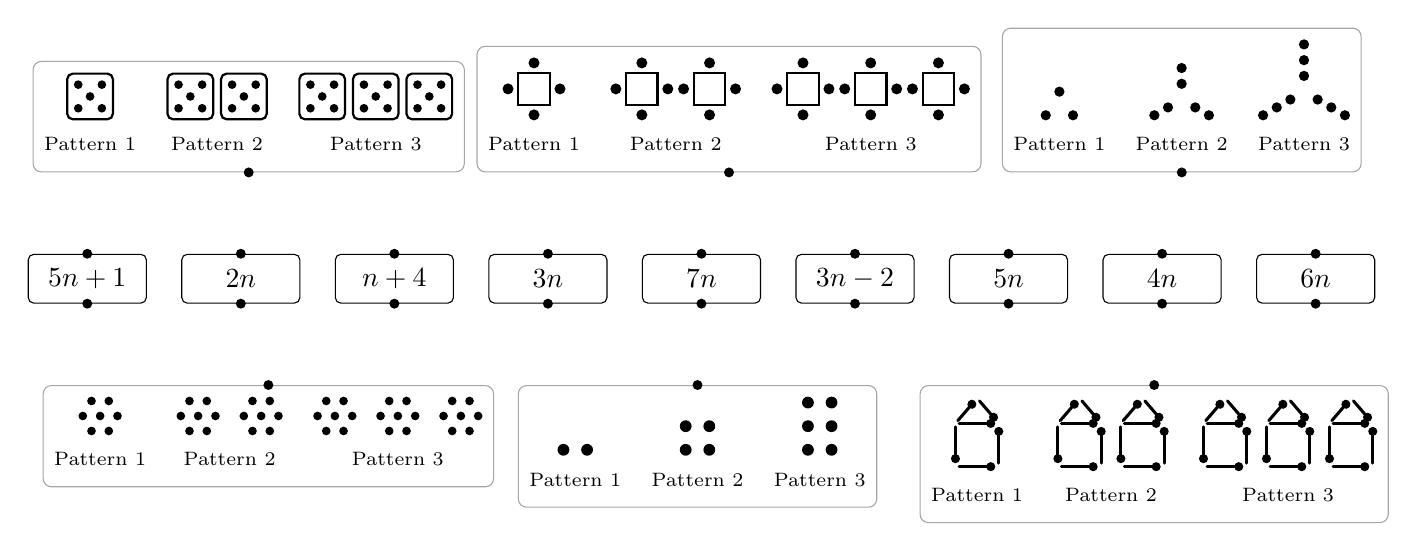
\begin{tikzpicture}[
    tile/.style={draw,rounded corners=2pt,minimum height=0.62cm,minimum width=1.5cm,inner sep=3pt},
    card/.style={draw=gray!70,rounded corners=3pt,inner sep=4pt}]
  \node[card,anchor=south] (A) at (2.8,1.35) {\threepatterns{\dicefives{1}}{\dicefives{2}}{\dicefives{3}}};
  \node[card,anchor=south] (B) at (8.9,1.35) {\threepatterns{\septables{1}}{\septables{2}}{\septables{3}}};
  \node[card,anchor=south] (C) at (14.65,1.35) {\threepatterns{\dotstar{1}}{\dotstar{2}}{\dotstar{3}}};
  \node[card,anchor=north] (D) at (3.05,-1.35) {\threepatterns{\dotflowers{1}}{\dotflowers{2}}{\dotflowers{3}}};
  \node[card,anchor=north] (E) at (8.5,-1.35) {\threepatterns{\dotrows{1}{2}}{\dotrows{2}{2}}{\dotrows{3}{2}}};
  \node[card,anchor=north] (F) at (14.3,-1.35) {\threepatterns{\sephouses{1}}{\sephouses{2}}{\sephouses{3}}};
  \foreach \x in {A,B,C} \fill (\x.south) circle (1.8pt);
  \foreach \x in {D,E,F} \fill (\x.north) circle (1.8pt);
  \foreach \i/\s in {0/{$5n+1$},1/{$2n$},2/{$n+4$},3/{$3n$},4/{$7n$},5/{$3n-2$},6/{$5n$},7/{$4n$},8/{$6n$}} {
    \node[tile] (T\i) at ({0.75+1.95*\i},0) {\s};
    \fill (T\i.north) circle (1.8pt);
    \fill (T\i.south) circle (1.8pt);}
\end{tikzpicture}
\end{center}

\item \ealpara{Narysuj wzory 1, 2 i 3 \ealkeytr{ciągu} obrazkowego dla każdego \ealkeytr{wzoru na n-ty wyraz}. Użyj zapałek, kropek lub innych przedmiotów.}{Draw patterns 1, 2 and 3 of a picture \ealkey{sequence} for each \ealkey{$n$th term}. Use matchsticks, dots or other objects.}
\ealpara{e) \ealkeytr{Wzór na n-ty wyraz} własny:}{e) An \ealkey{$n$th term} of your own:}
\ealpara{f) Czy można narysować \ealkeytr{wzór na n-ty wyraz} $-2n$? Wyjaśnij.}{f) Can the \ealkey{$n$th term} $-2n$ be drawn? Explain.}

\begin{tabular}{@{}l@{\hspace{10pt}}l@{}}
(a) \ $3n$ & (b) \ $5n$\\\noalign{\vspace{-8pt}}
\dotpaper{8.3}{2.9} & \dotpaper{8.3}{2.9}\\\noalign{\vspace{7pt}}
(c) \ $8n$ & (d) \ $\tfrac12n$\\\noalign{\vspace{-8pt}}
\dotpaper{8.3}{2.9} & \dotpaper{8.3}{2.9}\\\noalign{\vspace{7pt}}
(e) \ An \ealkey{$n$th term} of your own: \ansline & (f) \ Can the \ealkey{$n$th term} $-2n$ be drawn? Explain.\\\noalign{\vspace{-8pt}}
\dotpaper{8.3}{2.9} & \dotpaper{8.3}{2.9}
\end{tabular}
\setcounter{asn}{\value{enumi}}
\end{enumerate}

\newpage
\parttitle{6}{Always, sometimes or never? (optional)}

\ealpara{Zdecyduj, czy każde stwierdzenie jest zawsze prawdziwe, czasami prawdziwe, czy nigdy nie jest prawdziwe, i zakreśl swoją odpowiedź. Wyjaśnij, skąd to wiesz, w polu uzasadnienia. Dla „czasami” podaj jeden przykład, w którym stwierdzenie jest prawdziwe, i jeden, w którym jest fałszywe. W każdym stwierdzeniu $n$ jest \ealkeytr{pozycją}, więc $n$ wynosi 1, 2, 3, \ldots}{Decide whether each statement is always true, sometimes true or never true, and circle your answer. Explain how you know in the reason box. For sometimes, give one example where the statement is true and one where it is false. In every statement $n$ is a \ealkey{position}, so $n$ is 1, 2, 3, \ldots}

\ealpara{\ealkeytr{Wyraz} \ealkeytr{tabliczki mnożenia} 6 jest także \ealkeytr{wyrazem} \ealkeytr{tabliczki mnożenia} 3.}{A \ealkey{term} of the 6 \ealkey{times table} is also a \ealkey{term} of the 3 \ealkey{times table}.}
\ealpara{\ealkeytr{Wyraz} \ealkeytr{tabliczki mnożenia} 3 jest także \ealkeytr{wyrazem} \ealkeytr{tabliczki mnożenia} 6.}{A \ealkey{term} of the 3 \ealkey{times table} is also a \ealkey{term} of the 6 \ealkey{times table}.}
\ealpara{\ealkeytr{Wyraz} \ealkeytr{tabliczki mnożenia} 25\% jest większy niż 100\%.}{A \ealkey{term} of the 25\% \ealkey{times table} is more than 100\%.}
\ealpara{Dodanie 2 do każdego \ealkeytr{wyrazu} \ealkeytr{tabliczki mnożenia} daje inną \ealkeytr{tabliczkę mnożenia}.}{Adding 2 to every \ealkey{term} of a \ealkey{times table} gives another \ealkey{times table}.}
\ealpara{\ealkeytr{Wyraz} \ealkeytr{ciągu} $2n+1$ jest \ealkeytr{parzysty}.}{A \ealkey{term} of the \ealkey{sequence} $2n+1$ is \ealkey{even}.}
\ealpara{$-2n$ jest mniejsze niż $-n$.}{$-2n$ is less than $-n$.}
\ealpara{$3n$ jest większe niż $n+2$.}{$3n$ is greater than $n+2$.}
\ealpara{W \ealkeytr{ciągu} $3n+1$, podwojenie \ealkeytr{pozycji} podwaja \ealkeytr{wyraz}.}{In the \ealkey{sequence} $3n+1$, doubling the \ealkey{position} doubles the \ealkey{term}.}
\ealpara{Liczba, która jest \ealkeytr{wyrazem} zarówno $3n$, jak i $5n$, jest także \ealkeytr{wyrazem} $15n$.}{A number that is a \ealkey{term} of both $3n$ and $5n$ is also a \ealkey{term} of $15n$.}
\ealpara{Liczba krzeseł w wzorze z tych stołów jest \ealkeytr{parzysta}.}{The number of chairs in a pattern of these tables is \ealkey{even}.}
\ealpara{Liczba kropek w rzędzie tych kostek jest \ealkeytr{parzysta}.}{The number of dots on a row of these dice is \ealkey{even}.}
\ealpara{Wzór z tych \ealkeytr{sześciokątów} zużywa dokładnie 100 zapałek.}{A pattern of these \ealkey{hexagons} uses exactly 100 matchsticks.}

\begin{asntable}
\asnrow{A \ealkey{term} of the 6 \ealkey{times table} is also a \ealkey{term} of the 3 \ealkey{times table}.}
\asnrow{A \ealkey{term} of the 3 \ealkey{times table} is also a \ealkey{term} of the 6 \ealkey{times table}.}
\asnrow{A \ealkey{term} of the 25\% \ealkey{times table} is more than 100\%.}
\asnrow{Adding 2 to every \ealkey{term} of a \ealkey{times table} gives another \ealkey{times table}.}
\asnrow{A \ealkey{term} of the \ealkey{sequence} $2n+1$ is \ealkey{even}.}
\asnrow{$-2n$ is less than $-n$.}
\asnrow{$3n$ is greater than $n+2$.}
\asnrow{In the \ealkey{sequence} $3n+1$, doubling the \ealkey{position} doubles the \ealkey{term}.}
\asnrow{A number that is a \ealkey{term} of both $3n$ and $5n$ is also a \ealkey{term} of $15n$.}
\asnrow[\septables{1}\quad\septables{2}]{The number of chairs in a pattern of these tables is \ealkey{even}.}
\asnrow[\dicefives{1}\quad\dicefives{2}]{The number of dots on a row of these dice is \ealkey{even}.}
\asnrow[\sephexagons{1}\quad\sephexagons{2}]{A pattern of these \ealkey{hexagons} uses exactly 100 matchsticks.}
\end{asntable}

\vspace{4pt}
\stepcounter{asn}
\ealpara{\textbf{Q\theasn.} Zapisz własne stwierdzenie każdego typu o \ealkeytr{wzorach na n-ty wyraz}.}{\textbf{Q\theasn.} Write your own statement of each type about \ealkey{$n$th terms}.}
\ealpara{Zawsze:}{Always: \hrulefill}
\vspace{7pt}
\ealpara{Czasami:}{Sometimes: \hrulefill}
\vspace{7pt}
\ealpara{Nigdy:}{Never: \hrulefill}

\end{document}